\documentclass[11pt]{article}
\usepackage{graphicx}
\usepackage[legalpaper,landscape, margin=0.4in]{geometry}
\usepackage{multicol}
\usepackage{titlesec}
\usepackage[dvipsnames]{xcolor}

\titlespacing*{\subsection}
{0pt}{1ex plus 1ex minus .3ex}{0ex}
\titlespacing*{\subsubsection}
{0pt}{1ex plus 1ex minus .3ex}{0ex}
\titleformat{\subsection}
  {\normalfont\fontsize{10.5}{15}\bfseries}{\thesection}{1em}{}
  \titleformat{\subsubsection}
  {\normalfont\fontsize{5}{12}\bfseries}{\thesection}{1em}{}
\begin{document}
\pagenumbering{None}
\setlength{\columnsep}{1cm}
\begin{multicols*}{3}
\section*{CS2107 cheatsheet}\\
{\color{Purple} \rule{\linewidth}{0.5mm} }
\colorlet{link}{RubineRed!70!}
\subsection*{Diffie hellman}
prime and generator is known to everyone\\
Can achieve forward secrecy
\subsection*{Reference monitor}
Order of ACL\\
Check user $>$ member of the group $>$ other
\subsection*{Vulnerability via testing}
White box, black box\\
Fuzzing - send malformed inputs to discover vuln
\\
Accesses to objects: Observe (Read), Alter (Write), Action (Execute)\\
\\
(1)The owner of the object decides the rights. (known as 
discretionary access control)
(2)A system-wide policy decides.  (known as mandatory access 
\subsection*{ Intermediate control}
Fine grain to meet security boundaries that are easy to manage\\
Group - can only by created by root or by a privileged user\\
Role based - determined by the role and assign the permissions for the role (least privilege principle)\\
Protection ring - higher privilege has lower ring number\\
\\
\textrm{\textbf{ Biba and Bell-LaPadula}}\\
Bell lapadula: no read up/ no write down\\
Biba: no write up/ no read down\\
\\
Both: only read/ write to same level\\
\subsection*{Terms}
\textbf{IPSec}
“Internet Protocol Security (IPsec)
communications by authenticating
is a protocol suite for securing Internet Protocol (IP)
and encrypting each IP packet of a communication
session. IPsec includes protocols for establishing mutual authentication \\\\
\textbf{Typosquatting}
Phishing with a typo in domain name leading to attacker's site\\\\
\textbf{Pharming}
poison the dns server and redirects user to a different website that looks the same\\\\
\textbf{Zero day vulnerability}
Use patch to derive vulnerability\\
Known exploits that is released on the day of attack\\\\
\textbf{CVE}
Security vulnerability database\\\\
\textbf{Spamhaus}\\
The Spamhaus Project is an international organisation, based in both London and Geneva, founded in 1998 by Steve Linford to track email spammers and spam-related activity\\\\
\textbf{CERT}\\
Computer Emergency Response Team (CERT) A Computer Emergency Response Team (CERT) is a group of information security experts responsible for the protection against, detection of and response to an organization's cybersecurity incidents\\\\
\textbf{SingCert}\\
Computer Emergency response team\\\\
\textbf{SOC}\\
a centralized unit in an organization that monitors the IT systems and 
deals with security issues\\\\
\textbf{White hat}\\
Access to source code\\
\textbf{Black hat}\\
No access to source code\\
\textbf{Grey hat}\\
Combination of both\\
\subsection*{chmod}
\textcolor{link}{\url{https://www.linode.com/docs/guides/modify-file-permissions-with-chmod/}}\\\\
\textbf{Octal representation}\\
chmod 750[bit for setuid...] ~/example.txt\\
chmod u=rwx,g=rx,o=.\\
setuid (4), setgid (2), and sticky(1)\\
\\
Can also use s to denote setuid\\
runs as the user who owns the executable file instead of the user who invoked the program to access sensitive information\\
\textcolor{link}{https://unix.stackexchange.com/questions/28363/whats-the-difference-between-s-and-s-in-ls-la}\\\\
Effective UID is root is owner is root
\subsection*{ps}
PID 1 is actively reserved for the init process to maintain consistency with older systems\\
\textcolor{link}{https://en.wikipedia.org/wiki/Process\_identifier}\\
\subsection*{Linux file permissions}
drwxr-xr-x\\
first character indicates whether it is a file or directory\\
Date is the date of last modification
\subsection*{Buffer overflow}\\
\%p points to a pointer (address)\\
\subsection*{Hash functions}
SHA256 needs to protect both the public key and private key
\subsection*{Birthday attack}
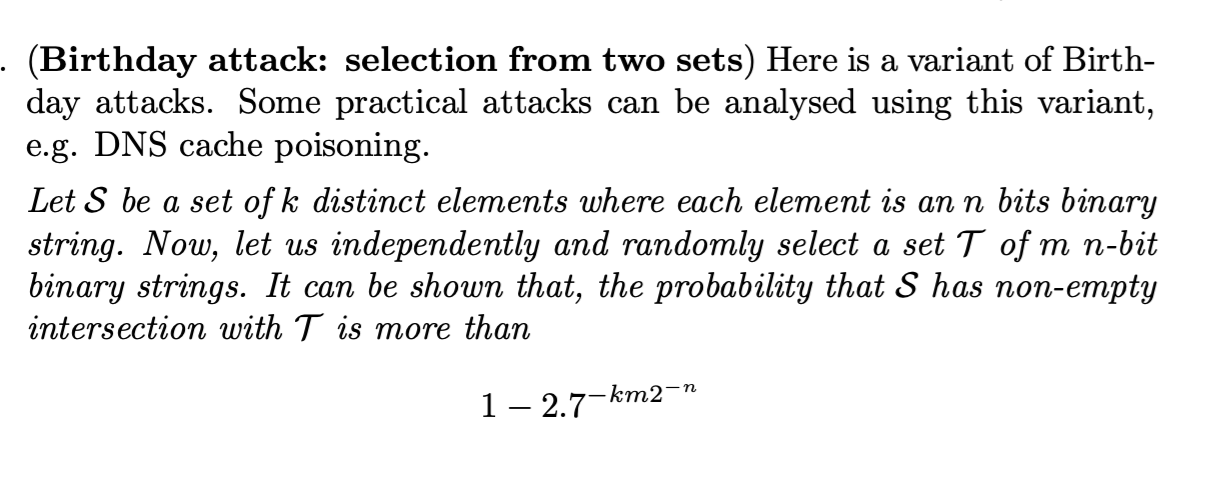
\includegraphics[height=3cm]{ss1}
\\
M $>$ 1.17 \sqrt{T}
\subsection*{Unilateral Authentication}
Generates a session key pair $<$k, t$>$ by verify the authenticity using the entity's public key\\\\
Related: MiTM,\\
When message is sent from Alice to Bob, decrypt using $k_{a}$ and encrypt using $k_{b}$\\
\subsection*{Strong Authentication - Challenge/Response}
Use shared secret key to generate mac, verification on receipt\\
mac is used against weak authentication to prevent sniffing
\subsection*{MAC vs hash}
MAC provides authenticity and hash provides integrity\\
Encryption provides confidentiality (not authenticity and integrity), a MAC provides integrity\\
Hash verifications and digital signatures can help ensure that transactions are authentic
\subsection*{Nonce}
Random number used in unilateral authentical using PKC to prevent replay attacks\\
Record everything and replay what the attacker has seen before\\
64-bit is more than sufficient to prevent the attacker from seeing a repeated nonce, need to observe large number of historical communication\\
\subsection*{PKC}
1.Alice choose a nonce\\
2.Bob signs r with private key, also attaches his certificate\\
3.Alice verifies the certificate, extract public key and verify that signature is correct
\subsection*{PKI}
standardised system that distributes public key\\
Uses certificates signed by CA to avoid online access to CA and to prevent CA from being a bottleneck\\
\subsection*{Certificate Structure}
(i) Name of an entity \\
(ii) Public key \\
(iii) Expiry data \\
(iv) Signature\\
Can obtain sender's public key from certificate\\
\\
\textbf{Self signed certificate}\\
Signed using entity's private key\\\\
\textbf{Encryption - Stream Cipher}\\
AES Counter mode\\\\
$msg_{0}$ and $mac_{0}$ \\
$ mac_{0}$ = (IV $\|$ xor cipher)\\
$mac_{1}$ can be forged with (IV $\|$ xor cipher XOR H(msg))\\\\
\textbf{RSA}\\
Subjected to factorization search is e is  65536 and below\\\\
\textbf{Renegotiable attack - TLS}\\
Client is connected to attacker server that connects with the actual server\\
Can be mitigated using CSRF token\\
Key for the first handshake encrypts the second handshake\\
Does not compromise confidentiality\\
Disabling renegotiation affects availability
\subsection*{MiTM}
Basic key exchange cannot guard against mallory\\
Communication from Alice is encrypted using $k_{a}$. mallory can decrypt using $k_{a}$ and re-encrypt using $k_{b}$.
Can see and modify the message\\
Remedy to use authenticated key exchange like PKC-based authenticated key-exchange\\
Outcome of authentication is a shared secret k (session key)\\
Example scheme is station-to-station protocol (sign the communication)\\
For mutual authentication, signing and verification is done by both ends
\subsection*{XSS}\\
exploit client's trust on the server\\
\textcolor{link}{https://owasp.org/www-community/xss-filter-evasion-cheatsheet}\\\\
\subsection*{XSRF}\\
exploit server's trust on the client
\textbf{Kerckhoff ’s principle}\\
adversaries know the
algorithm and format of the token\\
Replace with MAC
\\\\
\subsection*{RFC4086 recommendations}\\
Password At least 30 bits to be secure against online attacks, 60 bits against offline attacks \\
\subsection*{NIST recommendations}\\
Password 128 bits against offline attacks 
\subsection*{Cracking Dmgs}
\textcolor{link}{https://www.whitehatsec.com/blog/cracking-aes-256-dmgs-and-epic-self-pwnage/}
\\
\subsection*{Compiling source code}
John the ripper can crack /etc/shadow, break dmg\\
\textcolor{link}{https://dfir.science/2014/07/how-to-compiling-john-ripper-to-use-all.html}\\
\\./dmg2john your\_file.dmg $>>$ output
\\./john output]\\
or ./john - -format=dmg-opencl output\\
\\
View Makefile.in using nano, it asks to run with ./configure && make\\
\textcolor{link}{https://stackoverflow.com/questions/30805803/how-to-create-link-to-directory-in-makefile-in-linux}\\
\\
Can find more of the commands for pen test here\\
\textcolor{link}{https://www.hackingarticles.in/category/penetration-testing/}
\subsection*{Heartbleed bug}\\
Send more than the length of the request
\textcolor{link}{https://www.csoonline.com/article/3223203/what-is-the-heartbleed-bug-how-does-it-work-and-how-was-it-fixed.html}
\subsection*{WPA2}
Variants of WPA2, LEAP and PEAP (safe against offline attacks, but not online attacks)\\\\
Happens at link and physical layer\\
Key reinstallation attack bypasses https with sslstrip protocol\\
Github allows attacker to bypass firewall\\\\
If communication is carried out, the person is not aware that communication has occured\\
Covert channel hides the communication as the attacker doesn't want others to know that the machine is compromised
\\\\
TLS protect app information, WiFi protect the routing information\\
Attacker unable to spoof the IP address with IPSec, can only know source and destination (need to modify OS)\\
IP address may not be unique on the web server, but it is not a problem as there is a subnet\\\\
HTTP is built on top of TLS, SSL is the predecessor of TLS\\\\
\textcolor{link}{https://www.quora.com/How-do-I-view-what-websites-are-accessed-using-my-router-and-Wi-Fi}
\subsection*{Firewall}
Stateful packet inspection\\
While a packet filtering firewall only examines an individual packet out of context, a stateful firewall is able to watch the traffic over a given connection, generally defined by the source and destination IP addresses, the ports being used, and the already existing network traffic.
\subsection*	{Drive-by download}
Any download that happens without a person's knowledge, often a computer virus, spyware, malware, or crimeware
\subsection*	{Canary}
Can detect stack overflow\\
ASLR (memory randomization) can decrease attacker's chance of success
\subsection*{Side channel attack}
Other well-known side channel attacks include spying on the power consumption of an electronic device to steal an encryption key, or acoustic attacks that record the sound of a user's key strokes to steal their passphrase.\\
\subsection*{Backdoor}
(Covert channel) Most backdoors use HTTP or HTTPS for communicating with their C&C servers, but this malware was communicating over DNS, ICMP, and HTTP protocols.
\\
DNS is considered covert
\subsection*{DNSSEC}
DNSSEC strengthens authentication in DNS using digital signatures based on public key cryptography. With DNSSEC , it\'s not DNS queries and responses themselves that are cryptographically signed, but rather DNS data itself is signed by the owner of the data
\subsection*{Ciphers}
DES can be exhaustively searched
\subsection*{Substitution cipher}
27! = log_{2}^{94} $\approx$ 94 bits if each letter is mapped to itself, $2^{94}$ loops \\
$27^k$ otherwise\\
\\
Known plaintext attack: has plaintext and ciphertext\\
\textbf{Ciphers affected}: Substitution, permutation cipher\\\\
Ciphertext only attack: frequency analysis\\
\textbf{Ciphers affected}: Substitution, permutation cipher
\subsection*{OTP}
encryption: plaintext XOR key\\
decryption: ciphertext XOR key
\subsection*{Block cipher}
DES/ AES \\
Mode of operation: dividing into blocks before applying block cipher\\
ECB and CBC are block cipher\\\\
CTR is a stream cipher (can be compute before we see the plaintext)\\
ECB applies same key\\
For CBC, each use a new IV, the ciphertext will be very long so it takes the value from the previous block, have to see everything to decrypt\\
r is the long pseudorandom sequence, use a short key to generate a long key
\subsection*{Stream cipher}
Long pseudorandom sequence is generated with secret key and IV
\subsection*{Meet in the middle}
Remedy using 3DES
\\
\subsection*{Secure programming}
Example: Privilege escalation attack\\\\
Format string bugs, use of variable args, function can accept any number of arguments (not type safe, no bounds check)\\
 can be spotted by simply counting the number of arguments passed to the function\\
 \\
\subsection*{Format String attack}
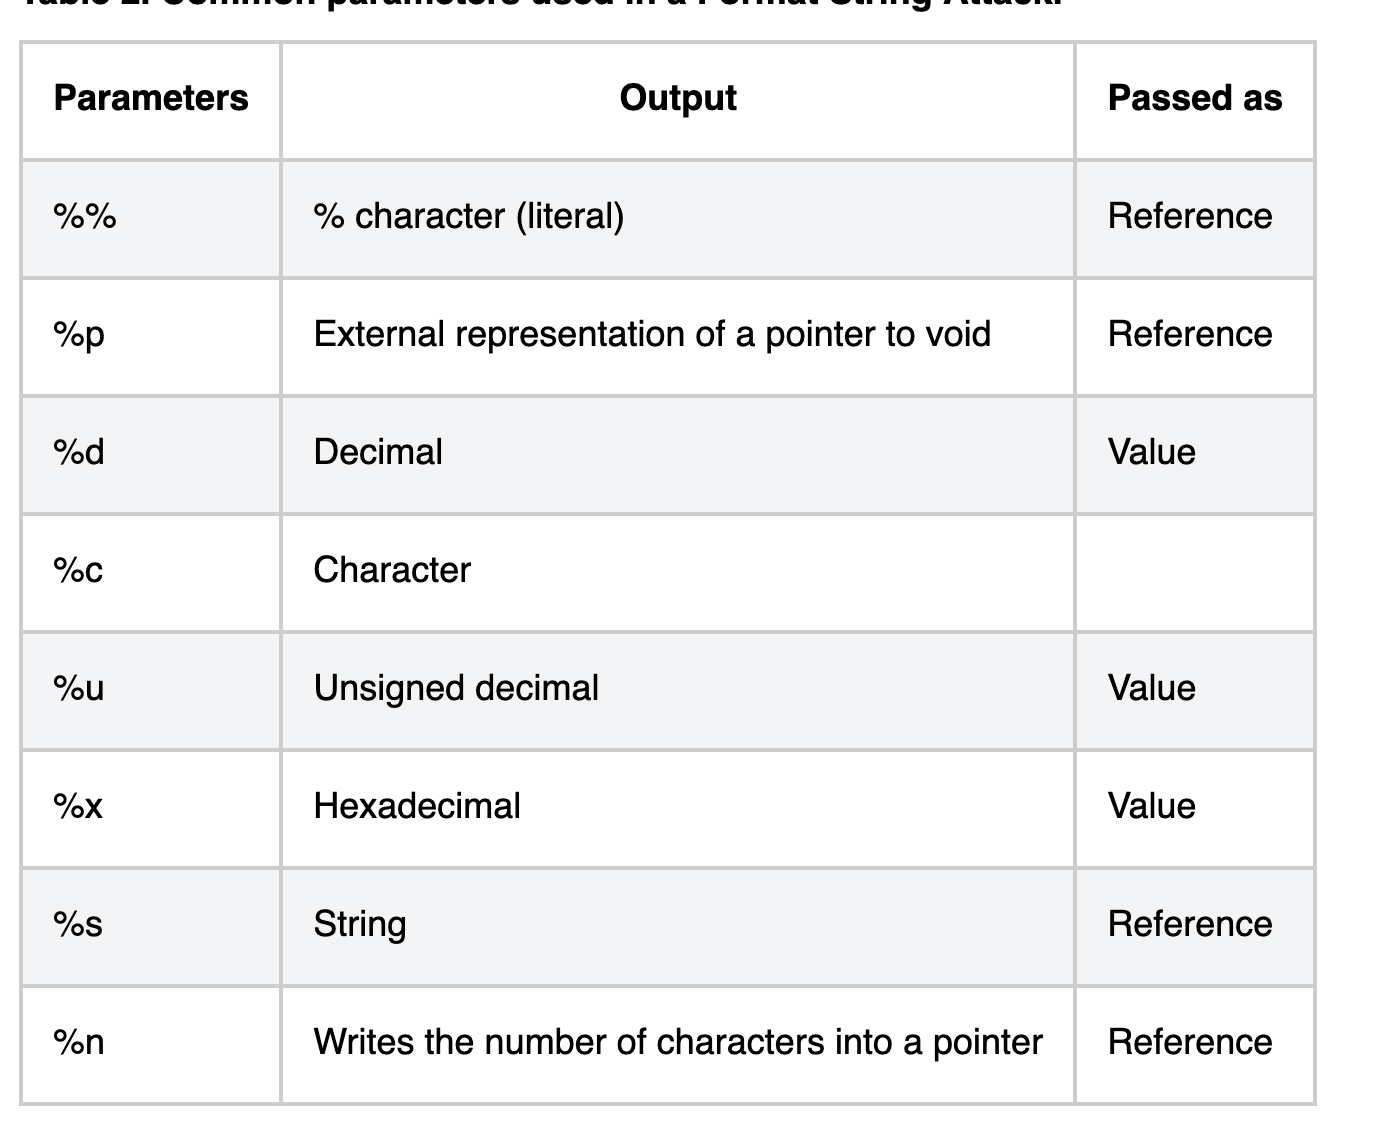
\includegraphics[height=5cm]{images/ss2}\\\\
\textcolor{link}{https://owasp.org/www-community/attacks/Format$_$string$_$attack}
\\\\
Display the address based on null termination and verifies based on non-null termination\\
luminus.nus.edu.sg$\backslash$0.attacker.com\\
\\
Overflow could inject attacker's shell code into memory $\rightarrow$ memory integrity lead to compromise of execution integrity\\
\subsection*{Same origin policy}
\textcolor{link}{https://www.acunetix.com/blog/web-security-zone/what-is-same-origin-policy/}
\\
Rule enforced by web browsers\\
origin is protocol,  hostname, and port number\\\\
\\Reflection XSS (non persistant)\\
malicious script coming from same origin (privilege escalation)\\
\\Stored XSS (persistant)
\\
XSRF: exploit server's trust on the client\\
Through clicking on the link which cannot run a script to get the authentication token
\\
To prevent CSRF attacks,\\
Use same-origin policy\\
\end{multicols*}

\end{document}
